\documentclass[12pt]%[english]
{article}

\usepackage{graphicx}
\usepackage{microtype}
\usepackage[nonumberlist, acronym, toc, section]{glossaries}
\usepackage{cite} 


\newglossary[slg]{symbolslist}{syi}{syg}{Symbols}

\makeglossaries

%commands for symbols
\newglossaryentry{symb:Pi}{
name=$\pi$,
description={You know it.},
sort=symbolpi, type=symbolslist
}
\newglossaryentry{symb:Phi}{
name=$\varphi$,
description={At vero eos et accusam et justo duo dolores et ea rebum..},
sort=symbolphi, type=symbolslist
}
\newglossaryentry{symb:Lambda}{
name=$\lambda$,
description={Lorem ipsum dolor sit amet, consetetur sadipscing elitr, sed diam nonumy.},
sort=symbollambda, type=symbolslist
}
 
%commands for abbreviations
\newacronym{MS}{MS}{Microsoft}
\newacronym{CD}{CD}{Compact Disc}

% ...

%abbreviations and glossary combined
\newacronym{AD}{AD}{Active Directory\protect\glsadd{glos:AD}}
 
% ... 
 
%glossary commands

\newglossaryentry{glos:AD}{
name=Active Directory,
description={At vero eos et accusam et justo duo dolores et ea rebum. Stet clita kasd gubergren, no sea takimata sanctus est Lorem ipsum dolor sit amet}
}

\newglossaryentry{glos:F}{name=File, description={An arbitrary file}}

% ...

\begin{document}

\begin{titlepage}

\begin{center}

{\Huge {
Term Paper Data Science 1}
}
\\[2ex]

\textbf{
\Large 
Docent: Prof. Dr. Lena Wiese \\ 
Semester: Summer Term 2021\\  
}




\includegraphics[scale=0.4]{logo.jpg} \\ 
\large{\textbf{Institute of Computer Science \\ Goethe-Universit\"at Frankfurt a. M.}}



\begin{tabular}{ll}
Authors: & \textsc{Franziska Hicking} \\
& {\small your Student ID} \\
& {\small your.email@ddre.ss} \\
& {\small branch of study (Bachelor/Master, semester count)} \\
& \textsc{Jonas Elpelt} \\
& {\small your Student ID}\\
&{\small  your.email@ddre.ss}\\
& {\small branch of study (Bachelor/Master, semester count)} \\
& \textsc{Julian Rummel} \\
&{\small  6673334}\\
& {\small s9594673@stud.uni-frankfurt.de}\\
&{\small  Master Bioinformatics, 2} \\
& \textsc{Niklas Conen}\\
& {\small 6599913}\\
& {\small conen@stud.uni-frankfurt.de}\\
& {\small branch of study (Bachelor Computer Science, 8)}\\
Date: & \today \\		
\end{tabular}

\end{center}

\vspace*{\fill}

\large
\noindent{}Chosen Project Topic: \\
T4 - DISTANCE MEASURES AND CLUSTERING


\end{titlepage}

\newpage\thispagestyle{empty}~ %empty page
\newpage 

\begin{abstract}
Lorem ipsum dolor sit amet, consetetur sadipscing elitr, sed diam nonumy eirmod tempor invidunt ut labore et dolore magna aliquyam erat, sed diam voluptua. At vero eos et accusam et justo duo dolores et ea rebum. Stet clita kasd gubergren, no sea takimata sanctus est Lorem ipsum dolor sit amet. Lorem ipsum dolor sit amet, consetetur sadipscing elitr, sed diam nonumy eirmod tempor invidunt ut labore et dolore magna aliquyam erat, sed diam voluptua. At vero eos et accusam et justo duo dolores et ea rebum. Stet clita kasd gubergren, no sea takimata sanctus est Lorem ipsum dolor sit amet. Lorem ipsum dolor sit amet, consetetur sadipscing elitr, sed diam nonumy eirmod tempor invidunt ut labore et dolore magna aliquyam erat, sed diam voluptua. At vero eos et accusam et justo duo dolores et ea rebum. Stet clita kasd gubergren, no sea takimata sanctus est Lorem ipsum dolor sit amet.   

Duis autem vel eum iriure dolor in hendrerit in vulputate velit esse molestie consequat, vel illum dolore eu feugiat nulla facilisis at vero eros et accumsan et iusto odio dignissim qui blandit praesent luptatum zzril delenit augue duis dolore te feugait nulla facilisi. Lorem ipsum dolor sit amet,
\end{abstract}

\newpage

\tableofcontents

\newpage


\section{Definition of Distance Measure}
\label{def_DM}

A distance measure is a function $d(x, y)$ that calculates a real value between two points in a space, containing two sets of points. This function must satisfy the four following axioms:
\begin{enumerate}
\item No negative distances:\\
$d(x, y) \geq 0$
\item Identity of indiscernibles:\\
$d(x, y) = 0$, iff $x = y$
\item Symmetry: \\
$d(x, y) = d(y, x)$
\item Triangle inequality: \\
$d(x, y) \leq d(x, z) + d(z, y)$
\end{enumerate}
The triangle-inequality impose the condition that a distance reflects the shortest path between two points. Thus, it is not possible to achieve a distance improvement by traveling via an intermediate point $z$. \cite{MMDS}

\section{Different Distance Measurements}

\subsection{Euclidean Distances}
The Euclidean distance calculates the distance of two points, represented as vectors of $n$ real numbers, in an $n$-dimensional euclidean space. In general, a Euclidean distance measure $d$ is called $L_r$\textit{-norm}, for arbitrary constants r. 
$$d([x_1,x_2,...,x_n], [y_1,y_2,...,y_n])=\sum_{i=1}^{n}(|x_i-y_i|^r)^\frac{1}{r}$$
The typical euclidean norm refers to the $L_2$\textit{-norm} and is calculated as the positive square root of the sum of all squared distances in each dimension.
$$d([x_1,x_2,...,x_n], [y_1,y_2,...,y_n])=\sqrt{\sum_{i=1}^{n}(|x_i-y_i|)^2}$$
It is simple to verify three of the aforementioned axioms (\ref{def_DM}).
\begin{enumerate}
\item No negative distances:\\
The nonnegative values are given by the positive square root. let $x \neq y$, then the square of any real number is always positive.
\item Identity of indiscernibles:\\
For $x = y$ the value is obviously $0$. Let $x = y$, then $(|x - y|)^2 = 0$ and $\sqrt{0} = 0$.
\item Symmetry: \\
Symmetrie is cleary given by the square of each distance.\\
$(x - y)^2 = (y - x)^2$.
\item Triangle inequality: \\
As a matter of fact, this axiom requires a more difficult proof. However, to keep it simple, the Euclidean space possesses the property that the sum of the lengths of Cathetus and Ancathetus is always longer than the length of the Hypothenuse. \cite{MMDS}
\end{enumerate}

\subsection{Cosine Distance}
The angular cosine distance gives the (normalized) angle between two points $x$ and $y$ represented as vectors in an $n$-dimensional space. It does not make a difference between a vector and a multiple of that vector. The cosine distance can be calculated by applying the arc-cosine function to the cosine of the angle $\theta$ between $x$ and $y$ \cite{MMDS}. \\
It is based on the cosine similarity (cosine between two vectors $x$ and $y$), which is definied as: \\

\begin{equation}
	\text{cosine similarity} = \frac{\sum_{i=1}^{n} x_i y_i}{\sqrt{\sum_{i=1}^{n} x_i^2 \sum_{i=1}^{n} y_i^2}}
\end{equation}  

The cosine similarity, however, is not a distance as it is defined for positive values only. Therefore it has to be converted to the normalized angle between $x$ and $y$ as followed \cite{cosdist}: \\

\begin{equation}
	\text{angular cosine distance} = \frac{\arccos({\text{cosine similarity})}}{\pi}
\end{equation}  

Note, that if $x$ or $y$ are zero vectors, the cosine similarity would not be defined. To prevent a division by zero the cosine similarity is set to 1 in this special case (based on the implementation of the pairwise distance in scikit-learn). 

The axioms for a distance measure are fulfilled for the cosine distance \cite{MMDS}: \\

\begin{enumerate}
	\item Identity of indiscernibles:\\
	Two vectors can have a cosine distance of 0 if and only if they are located in the same direction. (This applies also to vectors that are multiples of one another and therefore are in the same direction.) 
	\item Symmetry: \\
	Symmetry is obviously given by the equality to measure an angle between $x$ and $y$ and an angle between $y$ and $x$. 
	\item Triangle inequality: \\
	A rotation from $x$ to $y$ can be explained by a rotation from $x$ to $z$ and then to $y$. Therefore a sum of these two rotations is always bigger or equal than the rotation directly from $x$ to $y$ 
	\item No negative distances:\\
	Regardless of the dimensionality of the space the values of the cosine distance are between 0 and 180 degrees, therefore no negative distances can occur. 
	
\end{enumerate}



\section{Data Set Description}

\subsection{Solar Flare}
The solar flare dataset is taken from the UCI Machine Learning Repository \cite{Dua2019}. Each point contains data recorded for on active region of the sun.
The first three attributes are the McIntosh classification of sunspot groups:
\begin{enumerate}
    \item Z-value: modified Zurich sunspot class, $\{A, B, C, D, E, F, H\}$
    \item p-value: description of the penumbra of the largest spot. A penumbra is a part of a sunspot that is darker than the suns surface. $\{x, r, s, a, h, k\}$
    \item c-value: description of the distribution of sunspots in a group $\{x, o, i, c\}$
\end{enumerate}
A detailed descriptions of the letter codes can be found in the original paper by McIntosh \cite{McIntosh1990}.
The following entries are as follows:
\begin{enumerate}
    \setcounter{enumi}{3}
    \item Activity (1: reduced, 2: unchanged)
    \item Evolution (1: decay, 2: no growth, 3: growth)
    \item Code for the previous 24h flare activity
    \item Is the region historically complex? (1: yes, 2: no)
    \item Todoooooo
    \item Area (1: small, 2: large)
    \item Area of the largest spot (1: $\geq 5$ deg$^2$, 2: $>5$ deg$^2$)
\end{enumerate}
The last three entries are a predicted flare classes 
\subsection{UCI ML Wine recognition dataset}
\marginnote{\textcolor{blue}{Jonas Elpelt}}
This dataset contains the chemical analysis results of Italian wines from 3 different cultivators. It is also taken from the UCI Machine Learning Repository \cite{Dua2019}. 
The dataset consists of 178 instances, each of them having 13 numeric attributes according to different measurements taken for different constitutuents (alcohol, malic acid, ash, alcalinity of ash, magnesium, total phenols, flavanoids, nonflavanoid phenols, proanthocyanins, color intensity, hue, OD280/OD315 of diluted wines, proline). Each instance belongs to either one of three classes containing 59, 71 and 48 data points. 
It was created by R. A. Fisher in July 1988 \cite{scikitlearn}. 

\section{Clustering Algorithms}
\subsection{K-Means}
\subsection{K-Medoids}
The K-Medoids clustering method is related to the well-known K-means algorithm, but uses medoids (representative points for each cluster) instead of means to define new cluster centers, which makes it more robust to outliers.\cite{Jin2010} It partitions the dataset by assigning each data point to the closest of $k$ cluster centers, which are defined by the most centrally located medoids. A medoid is a point with a minimal average dissimilarity to all other data points in the same cluster. The most commonly used algorithm to solve this NP-hard problem heuristically is the PAM (Partitoning Around Medoids) algorithm, that works as following: \cite{kaufman2009finding} \\
\begin{enumerate}
	\item First initialize the algorithm by selecting $k$ data points to be the medoids and assigning every data point to its closest medoid. \\
	\item Compare the average dissimilarity coefficient of a swap of each medoid $m$ and a non-medoid data point $\bar{m}$. Find a swap between $m$ and $\bar{m}$ that would decrease the average dissimilarity coefficient the most. 
	\item If no change of a medoid happened in the second step, terminate the algorithm, else re-assign the data points to the new medoids and go back to step 2. 
\end{enumerate}

\subsection{K-Median}
\subsection{DBSCAN}

DBSCAN was developed by Martin Ester, Hans-Peter Kriegel, Jiirg Sander and Xiaowei Xu. All following definitions and descriptions are taken from their original publication \cite{dbscan} or their revisit of DBSCAN \cite{dbscanrevisited} and only apply to this algorithm.\\
Contrary to the aforementioned centroid-based partitioning algorithms (k-means, k-medoids and k-median) the DBSCAN (\textit{Density Based Spatial Clustering of Applications with Noise}) algorithm uses point densities to determine clusters.\\
To introduce the definition of the density of a cluster, first the Eps-neighbourhood of a point is defined:\\
\ \\
\textbf{Definition 1:} \textit{Eps-neighbourhood}\\
A point q is part of the Eps-neighbourhood $N_{Eps}$ of point p if the distance between them is smaller than a threshold distance called Eps.\\
The Eps-neighbourhood therefore is defined as $N_{Eps} = \{q \in D \ | \ ||p, q|| \leq Eps \}$ with $D$ denoting the entirety of points that are supposed to be clustered and $||p, q||$ being the distance between p and q for an arbitrary distance measure.\\
\ \\
The Eps-neighbourhood fails at being a reliable measure for the point density if a point is located at the border of a cluster. These points are called \textit{border point}. Points that are located on the inside of a cluster are called \textit{core points}. Hence the following definition is made:\\
\ \\
\textbf{Definition 2:} \textit{directly density-reachable and density-reachable}\\
A point p is directly density-reachable from a point q when
\begin{enumerate}
    \item $p \in N_{Eps}(q)$
    \item $|N_{Eps}(q)| \geq \text{MinPts}$
\end{enumerate}
with \acrshort{minPts} being the minimal number of points that $N_{eps}(q)$ should contain so that q is considered a core point of a cluster.\\
A point is \textit{density-reachable} if there is a chain of points between $p$ and $q$ so that all neighbouring points in the chain are directly density reachable.\\
\begin{figure}[H]
    \centering
    \subfloat[eps-neighbourhood ]{{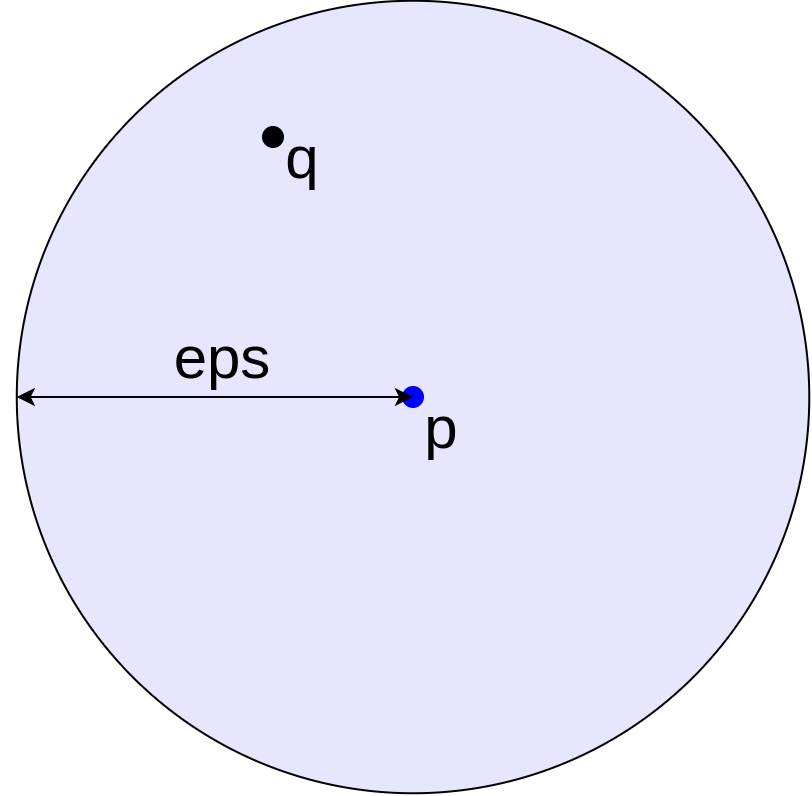
\includegraphics[height=7em]{./images/eps-neighbourhood}}}
    \qquad
    \subfloat[direct density-reachable]{{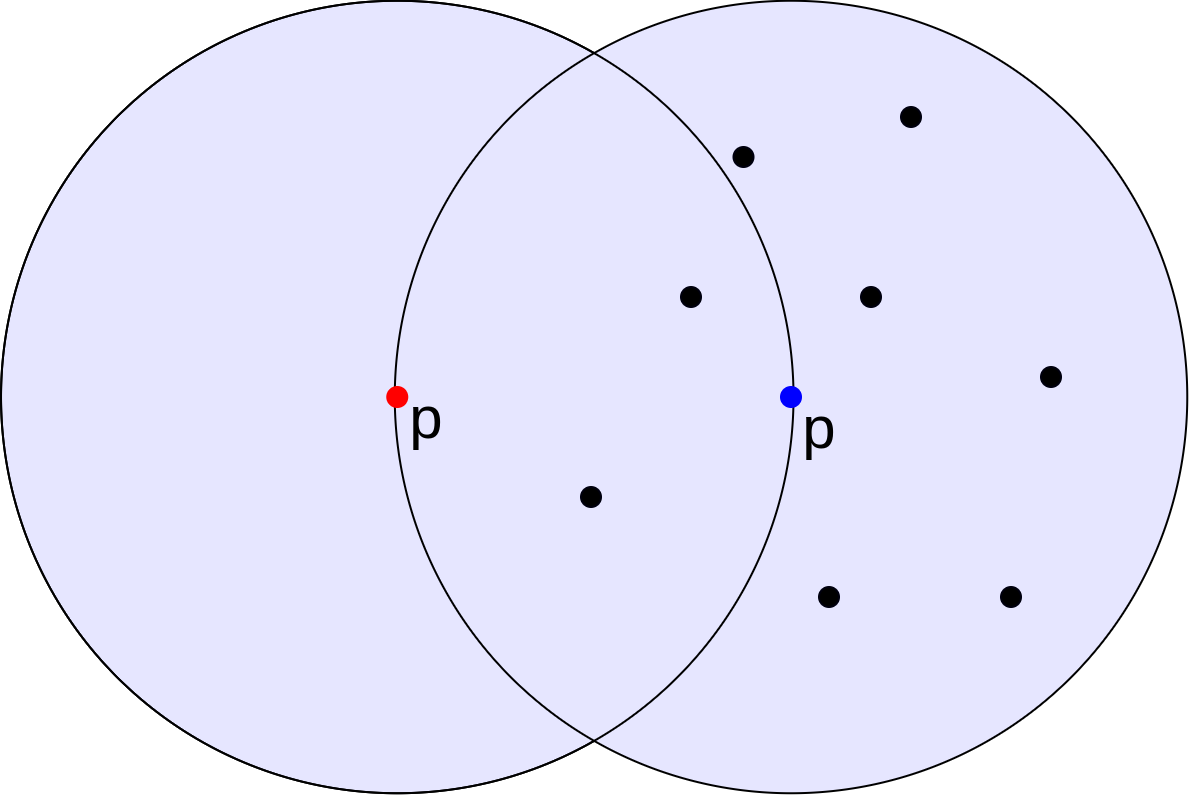
\includegraphics[height=7em]{./images/direct-density-reachable} }}
    \caption{visualisations of the definitions for eps-neighbourhood (left) and direct-density-reachable (right)}
\end{figure}
\ \\
To complete the definition of what is considered part of a cluster density-connectivity is defined:\\
\ \\
\textbf{Definition 3:} \textit{density-connected}\\
Two points $p$ and $q$ are considered density-connected if there is a common point $o$ which is density-reachable from $p$ and $q$.\\
\ \\
\begin{figure}[H]
    \subfloat[density-reachable]{{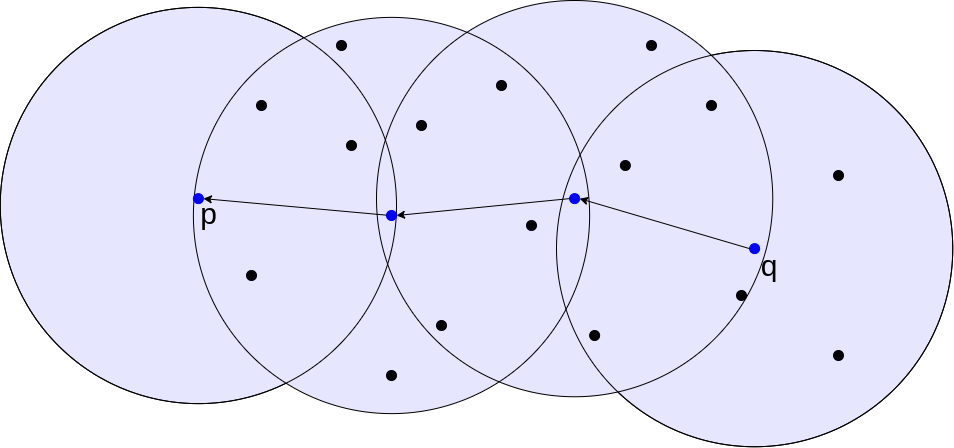
\includegraphics[height=7em]{./images/density-reachable} }}
    \subfloat[density-connected]{{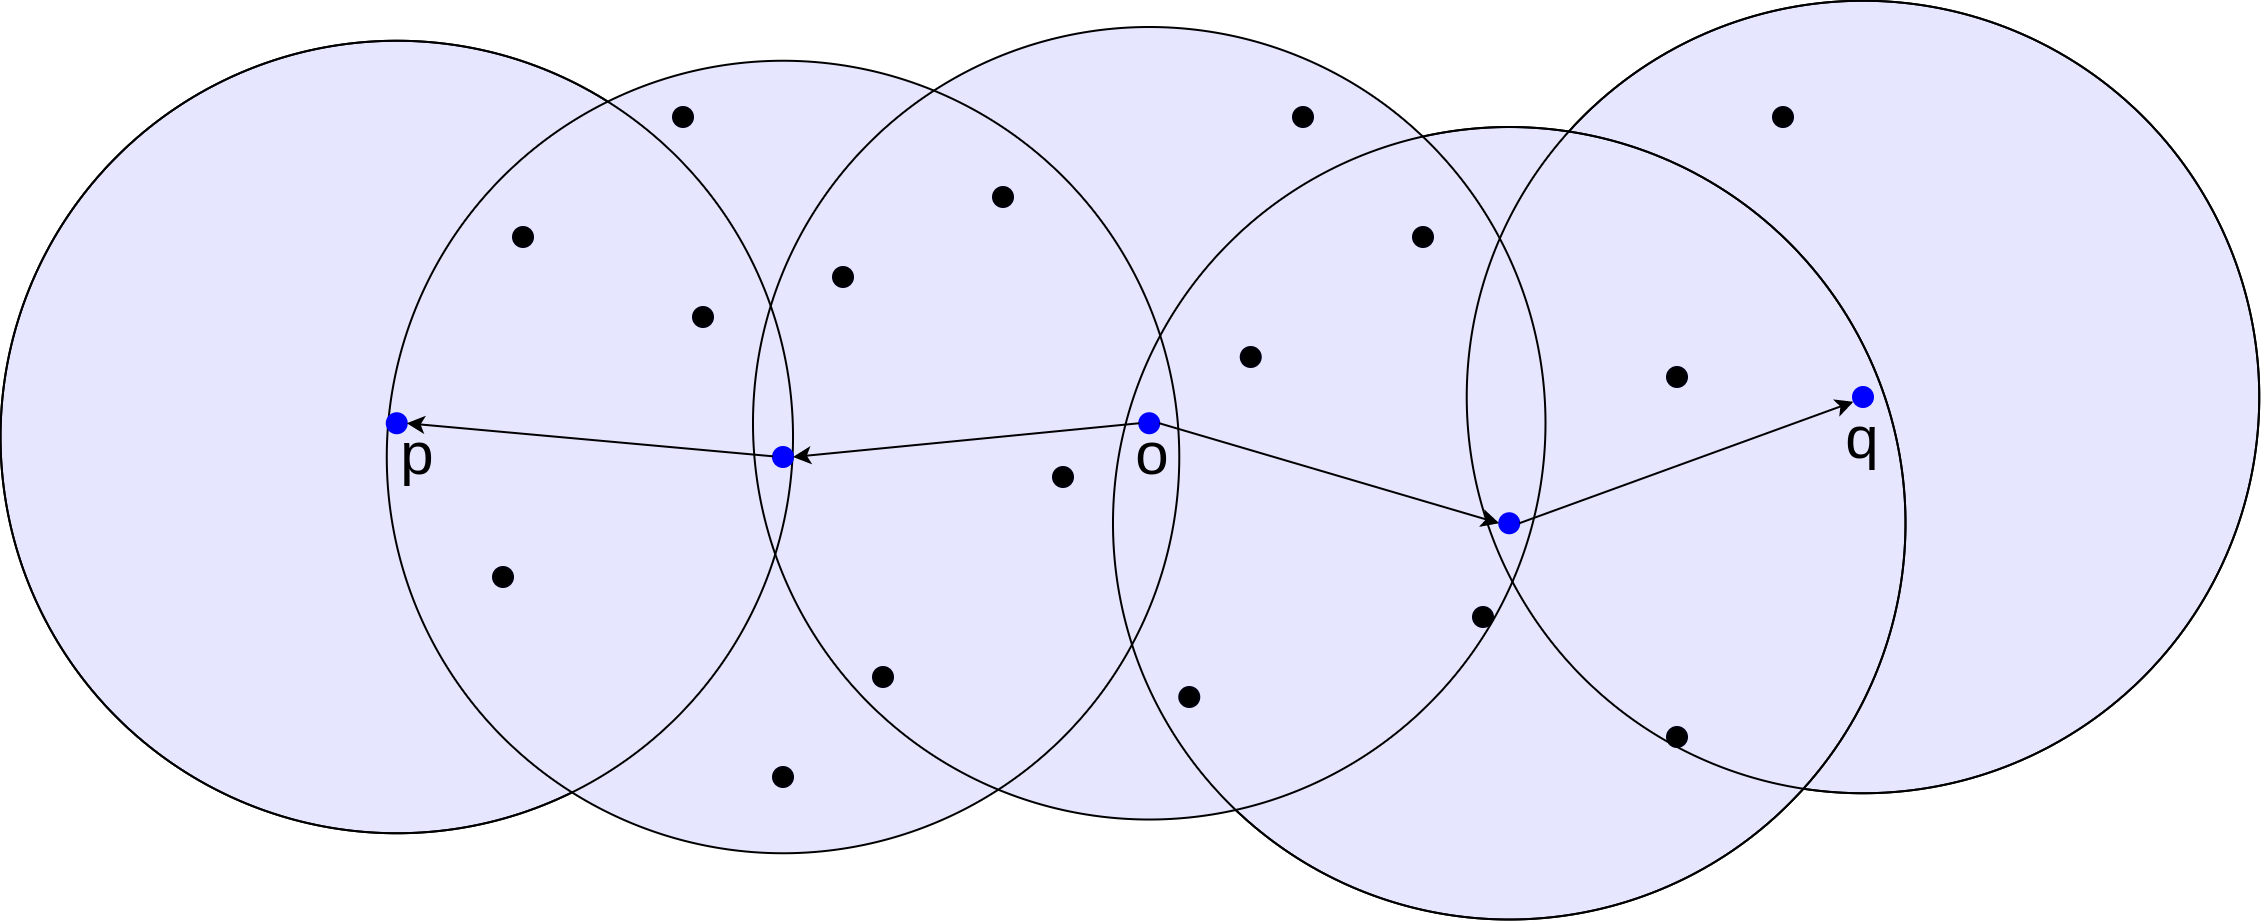
\includegraphics[height=7em]{./images/density-connected} }}  
    \caption{visualisations of the definitions for density-reachable (left) and density-connected (right)}
\end{figure}
Now a cluster can be described as:\\
\ \\
\textbf{Definition 4:} \textit{cluster and noise}\\
A cluster is a non empty subset $C \in D$ so that:
\begin{enumerate}
    \item $\forall p, q: p \in C \wedge q \text{ is density reachable from } p \Rightarrow q \in C$
    \item $\forall p, q \in C: \ p$ is density-connected to q
\end{enumerate}
\textit{Noise} is easily defined as every point that is not part of a Cluster $C_i$.\\
\ \\
Using these definitions DBSCAN can start the clustering process with given values for Eps and MinPts. First all points are marked as not labeled. Starting from an arbitrary point $p$ all points are iterated through in a linear fashion. For each point a \texttt{\Gls{glos:rangequery}} function is executed finding all directly density-reachable neighbours of $p$. If less then minPts neighbours are found, $p$ is labeled as noise. Otherwise $p$ is a core point and is labeled as part of the currently explored cluster. If this is the case the neighbourhood of $p$, from now on denoted as S, is expanded.\\
\ \\
Unlabled points get checked for the core point condition (which equals a \texttt{RangeQuery} call) and all subsequent found neighbours are also added to S. Points that got labeled as Noise beforehand and are part of S are labeled as part of the cluster.
When the expansion comes to an end a cluster is yielded, the next unlabeled point is chosen as $p$ and DBSCAN will continue to look for a new cluster.\\
\ \\
The biggest advantage of DBSCAN is its capability to find oddly shaped or spatially complex clusters. The aforementioned partitioning algorithms all fail at finding clusters that are not shaped like a sphere or a ellipsoid, if they are spatially entangled. scikit-learn published a great comparision of clustering algorithms on their website where the capabilities of DBSCAN are visualised \footnote{\url{https://scikit-learn.org/stable/auto_examples/cluster/plot_cluster_comparison.html}}. An example of DBSCANs capabilities generated using the python script on the aforementioned site is shown in figure \ref{fig:dbscanadv}.\\

Moreover DBSCAN allows for clustering without knowing the exact number of clusters or a termination criterion. Though finding the best values for minPts and eps can be equally challenging. The heuristic described in section \ref{dbscanheuristic} tries to simplify the estimation of these parameters.
\begin{figure}
    \centering
    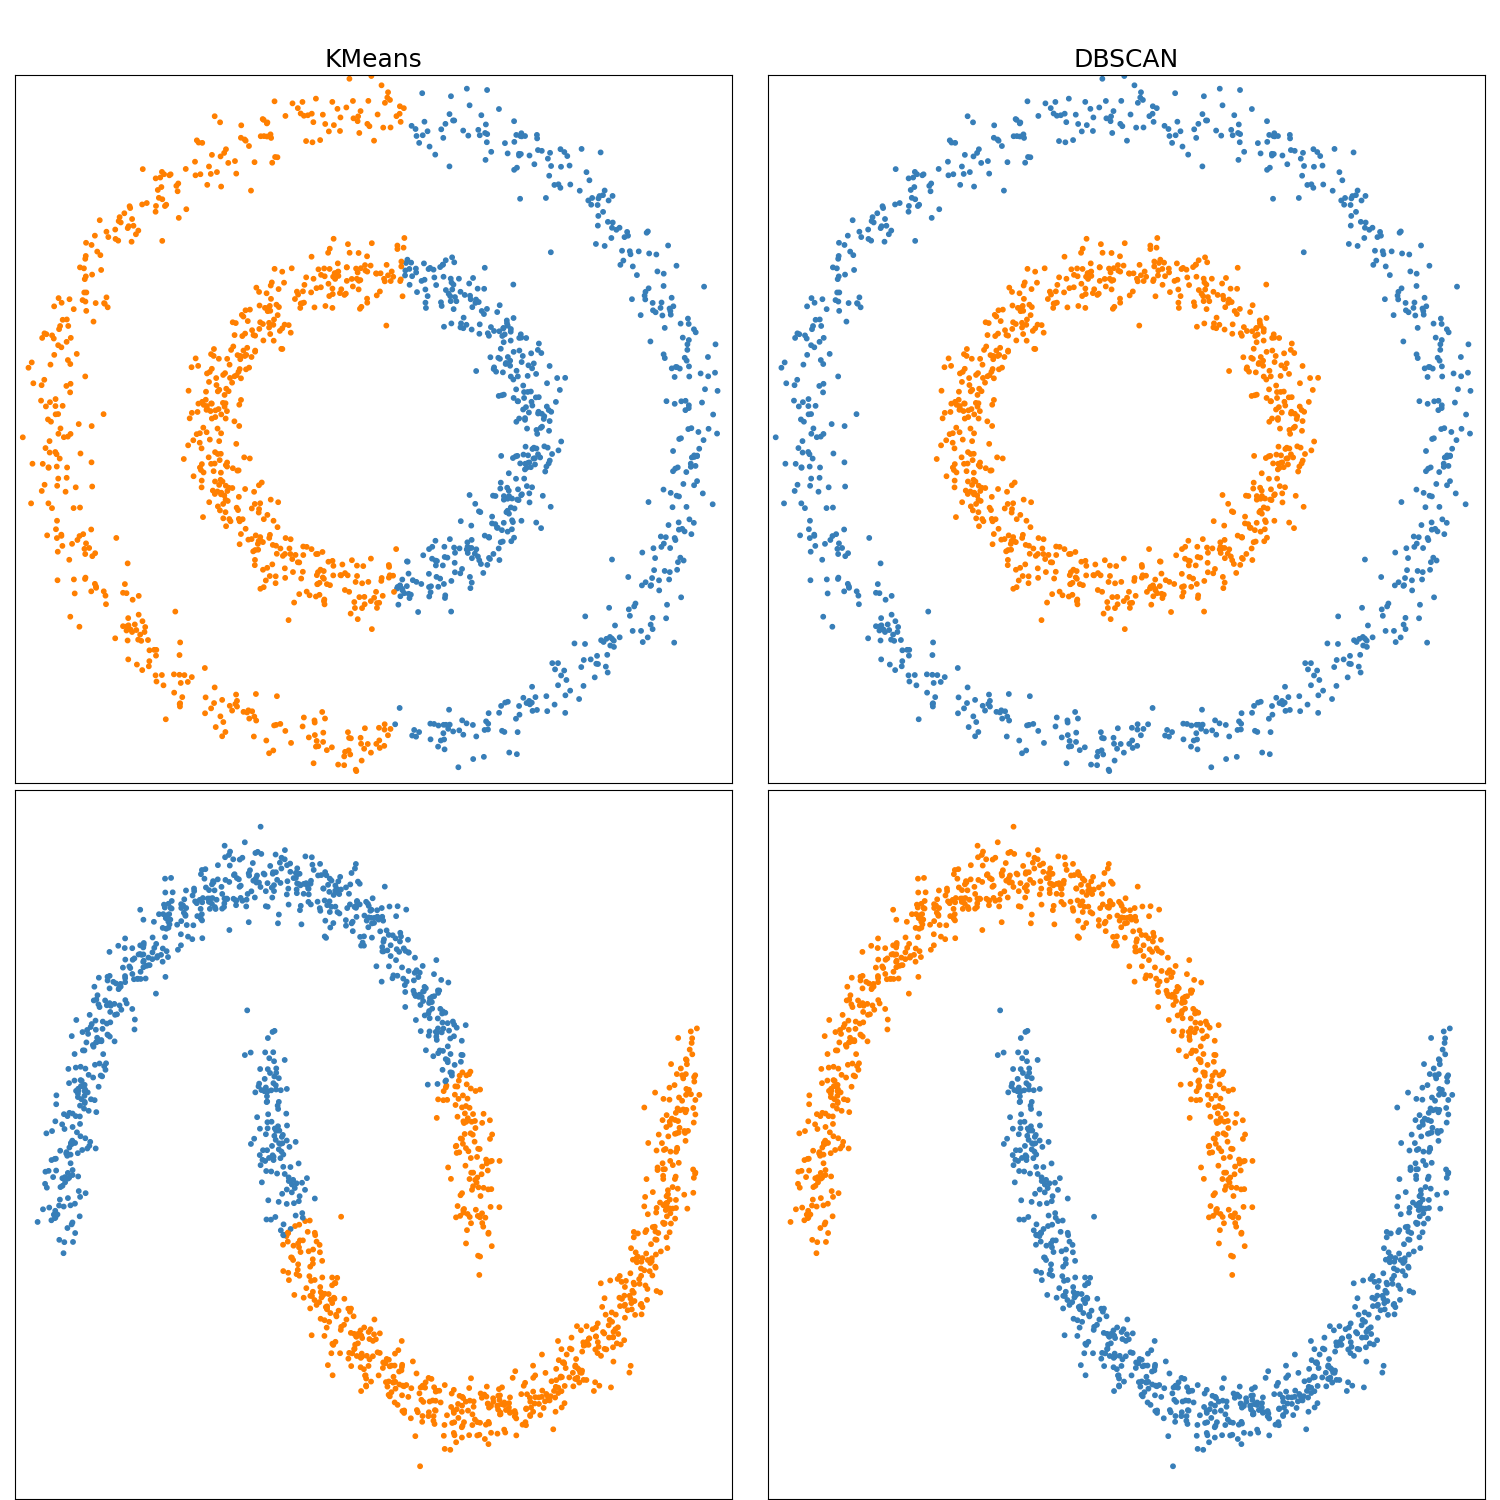
\includegraphics[width=0.4\textwidth]{../plots/dbscan/dbscan_comp}
    \caption{Comparision of DBSCAN to kmeans on spatially complex clusters}
    \label{fig:dbscanadv}
\end{figure}

Lastly DBSCAN will fail at finding multiple clusters if they are spatially close to each other. Because of the nature of the eps-neighbourhood all clusters with points seperated by a distance equal or less less than eps can not be distinguished.

The runtime complexity of DBSCAN heavily depends on the runtime of the \texttt{RangeQuery} function which is executed for every point in the dataset once.
If \texttt{RangeQuery} is implemented using a linear scan, its complexity will be $\Theta (n \cdot D)$ with $D$ being the time needed for calculating the distance between points. Therefore the runtime complexity of DBSCAN is $\Theta(n^2 \cdot D)$ \cite{dbscanrevisited}.


\section{Description of Python libraries used}
Libraries:
\begin{itemize}
\item pyclustering
\item sklearn
%The scikit-learn library \cite{scikit-learn} is used for loading the wine, iris and diabetis datasets and for clustering using the DBSCAN algorithm.
\end{itemize}

\section{Description of Evaluation Module}
ANMERKUNGEN:
\begin{itemize}
\item What are the results and how are they measured?
\end{itemize}

\section{Web Frontend and User Manual}
ANMERKUNGEN:
\begin{itemize}
\item Describe the implementation and write a brief user manual with screenshots.
\end{itemize}

\section{Conclusion}
ANMERKUNGEN:
\begin{itemize}
\item Summarize the main points and achievements
\item Add your own assessment/criticism on the topic
\end{itemize}

\newpage

%print glossary
\printglossary[style=altlist,title=Glossary]
 
%print abbreviations
\printglossary[type=\acronymtype,style=long]
 
%print symbols
\printglossary[type=symbolslist,style=long]

\newpage


\bibliography{bib.bib}
\bibliographystyle{unsrt}
\nocite{*}

\end{document}
